Llegada la etapa de implementación, hay que transformar a código lo analizado y diseñado en etapas anteriores. La petición que se nos hacía era que fuera una aplicación web, para ello se toman una serie de decisiones en cuanto a herramientas y lenguajes que se detallarán a continuación.

\section{Lenguajes}

Durante la carrera hay muy poca formación en cuanto a desarrollo web se refiere, solo una asignatura, que toca por encima el desarrollo en el lado del servidor con algunas nociones de PHP. La razón por la cual se elige entonces PHP para el desarrollo del proyecto es ampliar los conocimientos en dicho lenguaje, además de ser uno de los más usados, lo que implica que será sencillo encontrar solución a los posibles problemas que vayan apareciendo debido a la amplia documentación que hay disponible.\\

PHP es un lenguaje fácil de aprender, dado que posee mucha similitud con lenguajes como C, que si han sido aprendidos durante la carrera.\\

Tras comenzar el aprendizaje del lenguaje, surge el problema de que para hacer el desarrollo mínimamente organizado habría que implementar una serie de clases base que nos ayudaran con la implementación del sistema. Esto implica un trabajo tedioso que puede ahorrarse utilizando algún framework que nos proporcione herramientas que hagan mucho más fácil el trabajo. Es por ello que se decide utilizar {\em CodeIgniter}.
\\

{\em CodeIgniter} es un framework escrito en PHP, basado en el patrón arquitectónico MVC, a diferencia de otros frameworks existentes para PHP, es una herramienta realmente ligera, poco intrusiva y que facilita muchísimo el trabajo. Para ello pone a disposición algunas librerías y helpers, aumentando notablemente la productividad del desarrollador. \\

Otra gran ventaja de {\em CodeIgniter} es su documentación y su comunidad de desarrolladores, además de la Wiki en la que los usuarios van publicando plugins que pueden ser útiles para nuestro trabajo.\\

Uno de los problemas que encontramos con {\em CodeIgniter} es que a diferencia de otros frameworks MVC, no disponían de un ORM, es decir un sistema de persistencia que nos permitiera obtener elementos de la base de datos y transformarlos en objetos de nuestro sistema. Para ello se decide utilizar {\em Doctrine}, un ORM fácilmente integrable con {\em CodeIgniter}, y que nos permitía tener una base de datos virtual sobre nuestro sistema.\\

Pero la parte del servidor no es la única que hay que implementar, además necesitamos un lenguaje para las vistas. Para ello se elige XHTML, lenguaje de marcado ampliamente usado y recomendado por la W3C.\\

Otro objetivo es tener una buena interacción con el usuario, para ello es necesario el uso de un lenguaje que pueda interactuar con el DOM y modificarlo sin necesidad de pasar por el servidor, para ello elegimos JavaScript, soportado por la inmensa mayoría de navegadores. Se hace necesario para mejorar la interacción, el uso de una librería que facilite el trabajo con este lenguaje, para ello elegimos {\em jQuery}, la librería de JavaScript más usada, con multitud de plugins y una documentación muy bien estructurada.\\

\section{Extensiones y librerías}

El proyecto requiere la realización de algunas tareas complejas, como la generación de informes y la configuración de horarios, para ello se han utilizado una serie de librerías para obtener algunas funcionalidades difíciles de implementar. Éstas son:

\begin{itemize}

\item {\bf FullCalendar} - Plugin para {\em jQuery} que permite mostrar un calendario interactivo, con una API a disposición del desarrollador para responder a multitud de eventos, lo que permite una máxima personalización.
\item {\bf jQueryUI} - Plugin para {\em jQuery} con una gran variedad de widgets para mejorar la interacción con el usuario.
\item {\bf Farbtastic} - Plugin para {\em jQuery} que nos permite integrar un selector de color en una página.
\item {\bf FPDF} - Librería para PHP para la generación de documentos PDF.
\item {\bf PHPMailer} - Librería para PHP que facilita el envío de correos electrónicos.
\end{itemize}

\section{Herramientas utilizadas}

Para el desarrollo del proyecto se hace necesario el uso de una serie de herramientas, como editores de código, sistemas de control de versiones, etc. A continuación se detallarán todas las herramientas usadas en este proyecto.\\

La herramienta principal que se ha utilizado ha sido un IDE, en este caso {\em NetBeans} en su versión PHP. {\em NetBeans} es un entorno escrito en Java y pensado en un principio para desarrollar en este mismo lenguaje, pero conforme ha avanzado el tiempo se ha ido ampliando a más lenguajes, como por ejemplo PHP. La integración con este último es perfecta, proporcionando útiles herramientas como el autocompletado.\\

Para la detección de errores se hace casi obligado el uso de un {\em debugger}, en este caso hemos usado {\em XDebugger} que viene integrado en {\em NetBeans}, permitiendo utilizar puntos de ruptura en el código para comprobar el estado del sistema en un momento dado.\\

Para el despliegue de la aplicación se ha utilizado un entorno compuesto por un servidor {\em Apache}, base de datos {\em MySQL} y el intérprete de PHP, todo ello sobre un sistema GNU/Linux.\\

Otra herramienta utilizada que facilita el trabajo enormemente ha sido {\em Git}. {\em Git} es un sistema de control de versiones que facilita el desarrollo colaborativo y el mantenimiento de un software, versionando todos los cambios que se vayan produciendo en el código. Esto permite que si queremos volver a una versión anterior del sistema podamos hacerlo sin problema alguno, además de la creación de ramas de desarrollo, pudiendo fusionar ramas sin problema alguno.\\

\section{Detalles de la implementación de la arquitectura del sistema}

\subsection{Capa modelo}

Como hemos dicho, se ha utilizado la librería Doctrine como ORM. Esta librería sustituye completamente a la capa modelo del MVC de {\em CodeIgniter}, para ello, cada tabla de la base de datos se corresponde con un modelo. Para construir un modelo definimos sus atributos en una clase, además de sus relaciones, de esta forma, {\em Doctrine} generará automáticamente las tablas de la base de datos a partir de los modelos, aplicando todas las reglas de integridad definidas.\\

Un ejemplo de un modelo es el siguiente, que corresponde al de la tabla titulaciones:

\begin{lstlisting}[style=PHP]
class Titulacion extends Doctrine_Record
{
  public function setTableDefinition()
  {
    $this->setTableName('titulaciones');
    $this->hasColumn('id', 'integer', 4, array(
					       'type' => 'integer',
					       'length' => 4,
					       'primary' => true,
					       'autoincrement' => true,
					       'unsigned' => false,
					       'fixed' => false
					       ));
    $this->hasColumn('codigo', 'string', 4, array(
    					  'minlength' => 4,	
						  'length' => 4,
						  'notnull',
						  'notblank',						  
						  'unique',
						  'regexp' => '/[0-9]{4}/',
						  'unsigned' => false
						  ));
    $this->hasColumn('nombre', 'string', 200, array(
						    'type' => 'string',
						    'minlength' => 5,
						    'length' => 200,
						    'notnull' => true,
						    'unique' => true,
						    'notblank' => true,
						    'unsigned' => false
						    ));
    $this->hasColumn('creditos', 'integer', 4, array(
						     'type' => 'integer',
						     'length' => 4,
						     'unsigned' => true,
						     'notnull' => true,
						     'notblank' => true
						     ));
    $this->hasColumn('num_cursos', 'integer', 4, array(
                                'type' => 'integer',
                                'length' => 4,
                                'unsigned' => true,
                                'notnull' => true,
                                'notblank' => true
                             ));
  }

  public function getPlanificacion($id_curso)
  {
        $asignaturas = $this->asignaturas;
        $salida_total = array();
        foreach($asignaturas as $asignatura)
        {
            $q = Doctrine_Query::create()->select('c.*, p.*, a.descripcion')
                    ->from('PlanActividad p')
                    ->innerJoin('p.plandocente c')
                    ->innerJoin('p.actividad a')
                    ->where('c.id_curso = ? AND c.id_asignatura = ?', array($id_curso, $asignatura->id));
            $resultado = $q->execute();
            $salida = array();
            $salida[0] =  $asignatura->nombre;
            foreach($resultado as $actividad)
            {
                $salida[$actividad->id_actividad] = array($actividad->horas, $actividad->grupos, $actividad->horas_semanales);
            }
            $salida_total[] = $salida;
      }
      
      return $salida_total;
  }
  
  public function setUp()
  {
    parent::setUp();
    $this->hasMany('Asignatura as asignaturas', array('local' => 'id', 'foreign' => 'titulacion_id', 'onDelete' => 'CASCADE'));
  }
}
\end{lstlisting}

Como se puede ver en el código, se definen todos los atributos y sus reglas de integridad. En el método setUp definimos las relaciones, y además podemos definir nuestros propios métodos que devuelvan información personalizada de la base de datos.

\subsection{Capa controlador}

La capa controlador es la principal del sistema, la que recibe las peticiones, las procesa y las pasa a la vista para renderizar la página pedida. Al igual que en el modelo existe uno por cada subsistema.\\

Un controlador está compuesto de acciones, y cada una de ellas es llamada desde una URL del navegador, el controlador procesa la petición y realiza la lógica necesaria antes de devolver una respuesta, la estructura de un controlador es la siguiente:

\begin{lstlisting}[style=PHP]
class Titulaciones extends MY_Controller {

    function __construct() {
        parent::__construct();
        $this->titulaciones_table = Doctrine::getTable('Titulacion');
        $this->asignaturas_table = Doctrine::getTable('Asignatura');
        $this->layout = '';
        $this->notices = '';
        $this->alerts = '';
        $this->_filter(array('add', 'create', 'delete', 'edit', 'update', 'show_informes', 'show', 'exportar_planificacion'), array($this, 'authenticate'), 1); 
    }

    public function index() {

        $titulaciones = $this -> titulaciones_table -> findAll();

        //Conseguimos los items mediante el modelo
        $data['titulaciones'] = $titulaciones;
        $data['page_title'] = 'INDEX TITULACIONES';
        $data['enlace'] = 'titulaciones/show/';
        if($this -> input -> post('js') == '1') {
            unset($this -> layout);
            $this -> load -> view('titulaciones/_titulaciones', $data);
        } else {
            //Mostramos
            $this -> load -> view('titulaciones/index', $data);
        }
    }
\end{lstlisting}

Tenemos un constructor que es invocado en cada petición e inicializa algunos parámetros necesarios, y luego tenemos una acción, en este caso index, que busca todas las titulaciones en la base de datos y las pasa a la vista.

\subsection{Capa vista}

Esta capa es la que realmente ve el usuario, por tanto no es menos importante que las demás, aquí se utiliza un {\em layout} o plantilla por defecto que renderiza la parte que es común a todas las páginas, de forma que no se repite código en cada una de las vistas. Esta estructura común es la siguiente:

\begin{figure}[H] 
  \label{captura-layout} 
	\begin{center}
    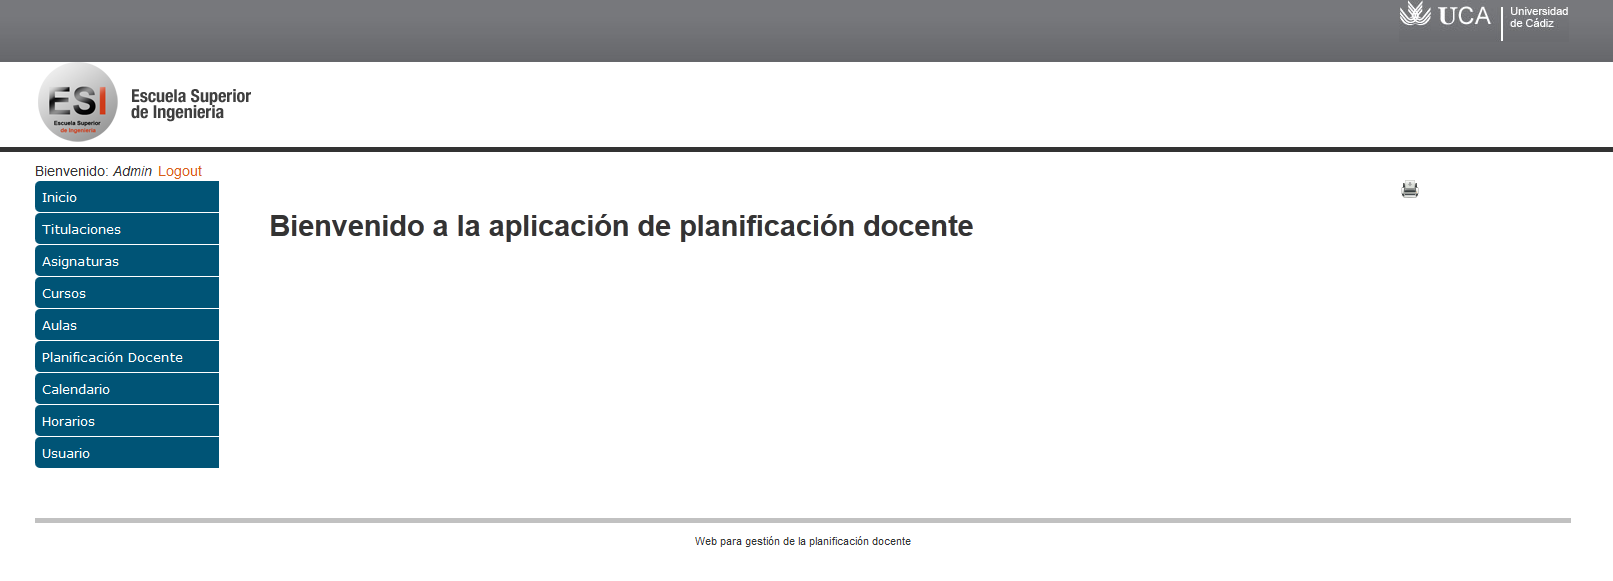
\includegraphics[scale=0.40]{./layout.png}
  \end{center}
\caption{Captura de la estructura de una página}
\end{figure}

En esta estructura tenemos un menú a la izquierda, una cabecera y un pié de página, además de un panel sobre el menú que indica el usuario que está conectado y permite su salida del sistema.\\

Todas las páginas siguen un estilo similar, por ejemplo una página que contiene una tabla de elementos, como esta con el listado de titulaciones:

\begin{figure}[H] 
  \label{captura-index-titulaciones} 
	\begin{center}
    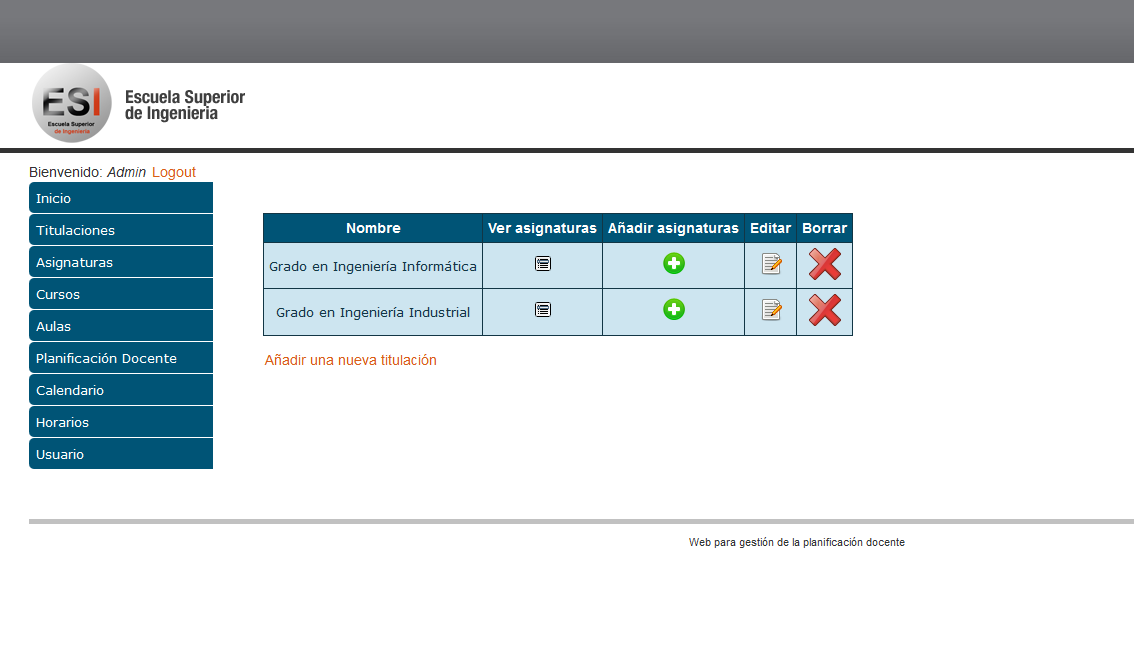
\includegraphics[scale=0.57]{./index-titulaciones.png}
  \end{center}
\caption{Captura del listado de titulaciones}
\end{figure}

La parte central del sistema es la gestión de horarios, para ello es necesaria una interacción sencilla con el usuario a la hora de construirlos y que no se convierta en una labor tediosa de realizar. Por ello se pensó que lo más sencillo sería arrastrar las asignaturas al lugar deseado en el horario, es decir, lo más intuitivo posible, esto es lo que veríamos en una de las páginas de configuración de horarios:

\begin{figure}[H] 
  \label{captura-horarios} 
	\begin{center}
    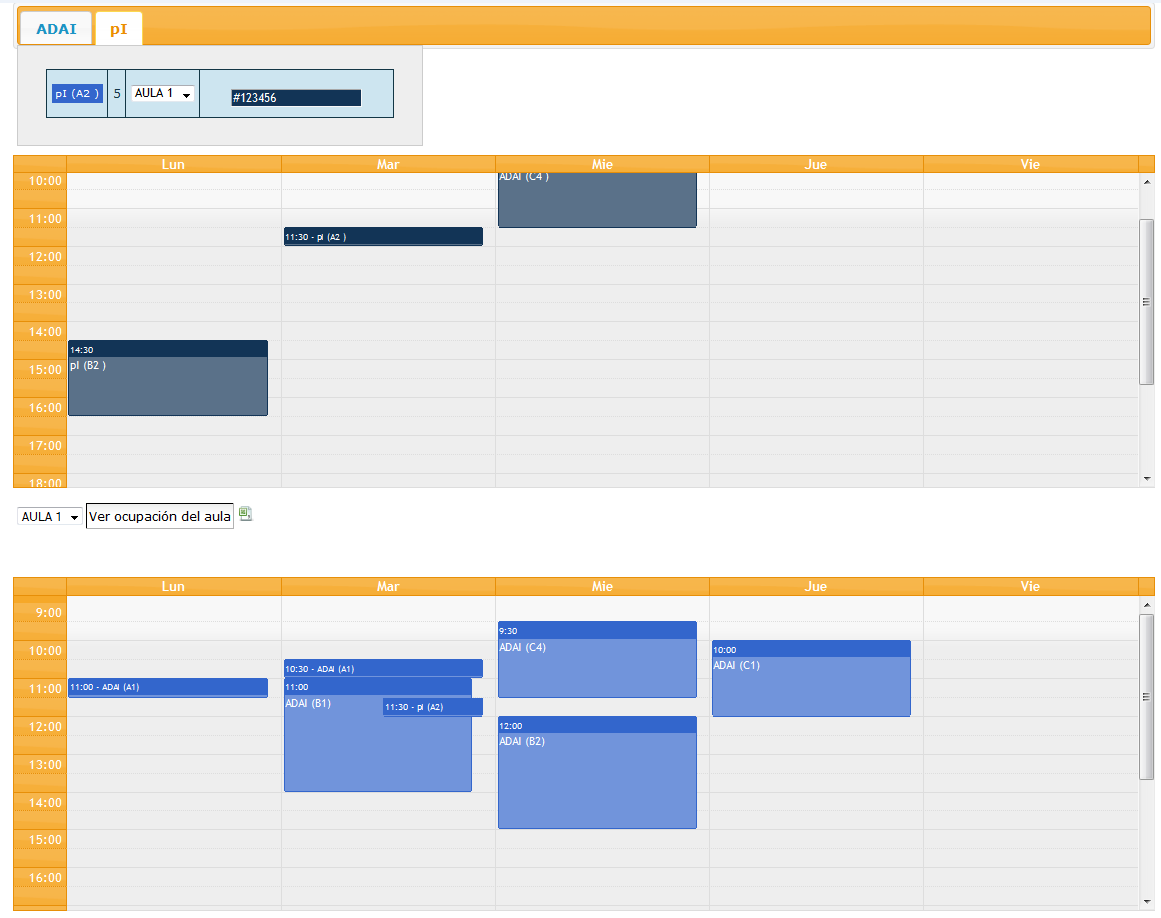
\includegraphics[scale=0.57]{./edit-horario.png}
  \end{center}
\caption{Captura de página de horarios}
\end{figure}

Tenemos tres partes diferenciadas en esta vista, un cuadro superior con las asignaturas aun no asignadas, que se podrán arrastrar al horario. Otra central con el horario de ese grupo, y otro bloque en la parte inferior en el que podemos ver la ocupación del aula que seleccionemos.\\

A la hora de asignar los slots en el horario hay que tener en cuenta diversos factores, como por ejemplo si el aula está ocupada, o si las asignaturas son solapables, para ello cada vez que se arrastra una asignatura al horario se hace una comprobación mediante la llamada a un servicio, devolviendo el resultado y dependiendo de si es satisfactorio o no, dejar la asignatura en su lugar o deshacer el cambio. Para deshacer el cambio, la API del plugin {\em FullCalendar} proporciona una función para invertir el proceso de la última acción realizada, eso hace el trabajo algo más sencillo.

